\documentclass[11pt]{article}
\usepackage{titling}
\usepackage{polski}
\usepackage[utf8]{inputenc}
\usepackage{fontspec}
\usepackage{setspace}
\usepackage{hyperref}
\usepackage{cite}
\usepackage{graphicx}

\setmainfont{Calibri Light}
\setstretch{1.15}
\setlength{\droptitle}{-5em}

\newenvironment{itquote}
  {\begin{quote} \begin{center}\itshape}
  {\end{center}  \end{quote}   \ignorespacesafterend}
  
\hypersetup{
  colorlinks=true,
  linkcolor=blue,
  urlcolor=cyan,
}
\urlstyle{same}


\setlength{\parindent}{0pt}
\setlength{\topmargin}{-1cm}
\setlength{\oddsidemargin}{-10pt}
\setlength{\textwidth}{480pt}
\setlength{\textheight}{600pt}

\author{Michał Puchyr}
\date{}
\title{\textbf{Czy dzisiejsza Polska wspiera przedsiębiorczość małych i średnich przedsiębiorstw?}}

\begin{document}
\maketitle
\section*{Wprowadzenie}
W dzisiejszych dynamicznych realiach gospodarczych, rola małych i średnich przedsiębiorstw (MŚP) w kształtowaniu stabilności ekonomicznej
oraz generowaniu innowacji staje się coraz bardziej kluczowa. Polska, będąca integralną częścią globalnej gospodarki,
nieustannie poszukuje skutecznych mechanizmów wspierania przedsiębiorczości w tej kategorii. Pytanie, czy dzisiejsza Polska
rzeczywiście wspiera rozwój MŚP, nabiera szczególnego znaczenia w kontekście dynamicznego rozwoju rynkowego,
zmieniających się warunków konkurencji oraz nieustannego dążenia do innowacyjności.

W niniejszej pracy podjęta zostanie próba zanalizowania polskiego krajobrazu biznesowego pod kątem dostępnych form wsparcia dla MŚP.
Dokonany zostanie przegląd różnorodnych programów rządowych, inicjatyw instytucji finansowych oraz struktur pomocowych, aby ocenić,
czy istniejące rozwiązania sprzyjają rozwojowi przedsiębiorczości w sektorze małych i średnich przedsiębiorstw.
Celem analizy będzie przegląd istniejących metod wspierania MŚP przez państwo a także ich ocena pod kątem efektywności i skuteczności.

\section*{Obecna sytuacja gospodarcza}
Polska gospodarka jest szóstą co do wielkości gospodarką w Unii Europejskiej i zarazem największą 
wśród członków Unii Europejskiej z krajów byłego bloku wschodniego \cite{RankingGospodarek}.
Przez ONZ jest uznawana za kraj wysoko rozwinięty pod względem wskaźnika rozwoju społecznego HDI który
bierze pod uwagę takie czynniki jak długość życia, średnią długość edukacji odbytej
przez 25-latków i oczekiwany czas edukacji dzieci w wieku szkolnym, jak również 
realny PKB per capita, tj. z uwzględnieniem siły nabywczej \cite{RankingHDI}.

W roku 2022 polska gospodarka stanęła przed trzema głównymi wyzwaniami. Pandemia COVID-19 nadal wpływała na 
funkcjonowanie przedsiębiorstw, rosyjska agresja na Ukrainę generowała napięcia geopolityczne, 
a kryzys energetyczny wprowadzał ograniczenia w dostawach energii, zwiększając koszty produkcji. 
Te czynniki skumulowanie stawiały Polskę przed trudnościami w utrzymaniu stabilności gospodarczej 
i wymagały elastyczności w dostosowywaniu się do zmieniającej się sytuacji.

\section*{Małe i średnie przedsiębiorstwa - definicja}
Definicja Małych i Średnich Przedsiębiorstw (dalej nazywana jako MŚP) została ustalona w 17 czerwca 2014 roku przez Komisję Europejską i jest stosowana w całej Unii Europejskiej.

Definicja przedsiębiorstwa według Komisji Europejskiej \cite{Komisja}

\begin{itquote}
  ``ZAŁĄCZNIK I

  \textbf{DEFINICJA MŚP}

  Artykuł 1

  \textbf{Przedsiębiorstwo}

  Za przedsiębiorstwo uważa się podmiot prowadzący działalność gospodarczą bez względu na jego formę prawną.
  Zalicza się tu w szczególności osoby prowadzące działalność na własny rachunek oraz firmy rodzinne zajmujące się rzemiosłem lub inną działalnością,
  a także spółki lub stowarzyszenia prowadzące regularną działalność gospodarczą.

  Artykuł 2

  \textbf{Pułapy zatrudnienia oraz pułapy finansowe określające kategorię przedsiębiorstwa}

  1. Do kategorii mikroprzedsiębiorstw oraz małych i średnich przedsiębiorstw („MŚP”) należą przedsiębiorstwa,
  które zatrudniają mniej niż 250 pracowników i których roczny obrót nie przekracza 50 milionów EUR, lub roczna
  suma bilansowa nie przekracza 43 milionów EUR.''
\end{itquote}

\section*{Rola MŚP w polskiej gospodarce}

Polska gospodarka, podobnie jak większość gospodarek, jest zdominowana przez mikroprzedsiębiorstwa.
Ich udział w strukturze wszystkich przedsiębiorstw wynosi aż 97,2\%. Mikroprzedsiębiorstwa mają największy, spośród wszystkich
grup przedsiębiorstw, udział w tworzeniu PKB - 29,5\% (dane za 2020 r.), a przyjmując wartość PKB generowaną
przez sektor przedsiębiorstw jako 100\% - 41,1\%. Podobnie wysoki udział charakteryzuje polskie mikrofirmy, gdy pod uwagę weźmiemy liczbę
pracujących w poszczególnych klasach wielkości przedsiębiorstw. Podmioty mikro generują 42,5\% miejsc
pracy w całym sektorze (liczba pracujących w takich firmach wynosi 4,3 mln osób). Większość mikroprzedsiębiorstw to firmy jednoosobowe, a przeciętna liczba
zatrudnionych w tej grupie podmiotów to ok. 1,5 mln osób \cite{RaportPARPoMSP}.

Sektor przedsiębiorstw wytwarza blisko trzy czwarte wartości PKB (71,6\%). Największy udział w tworzeniu
PKB mają mikroprzedsiębiorstwa - około 29,5\%. Cały sektor MSP generował 43,6\% PKB (dane za 2020 r.)\cite{RaportPARPoMSP}.

Wspieranie MŚP pomaga w tworzeniu klasy średniej, której źródłem utrzymania nie jest nisko kwalifikowana praca najemna
na niskich szczeblach drabiny organizacyjnej przedsiębiorstw.
\medskip

Analiza udziału przedsiębiorstw w tworzeniu PKB ze względu na sektor gospodarki pokazuje istotne różnice
pomiędzy dużymi przedsiębiorstwami a MSP. W przypadku MSP największe znaczenie miał sektor Usług, którego udział w tworzeniu PKB wyniósł
w 2020 r. 46,8\%, podczas gdy w dużych firmach - 30,1\%.

\begin{center}
  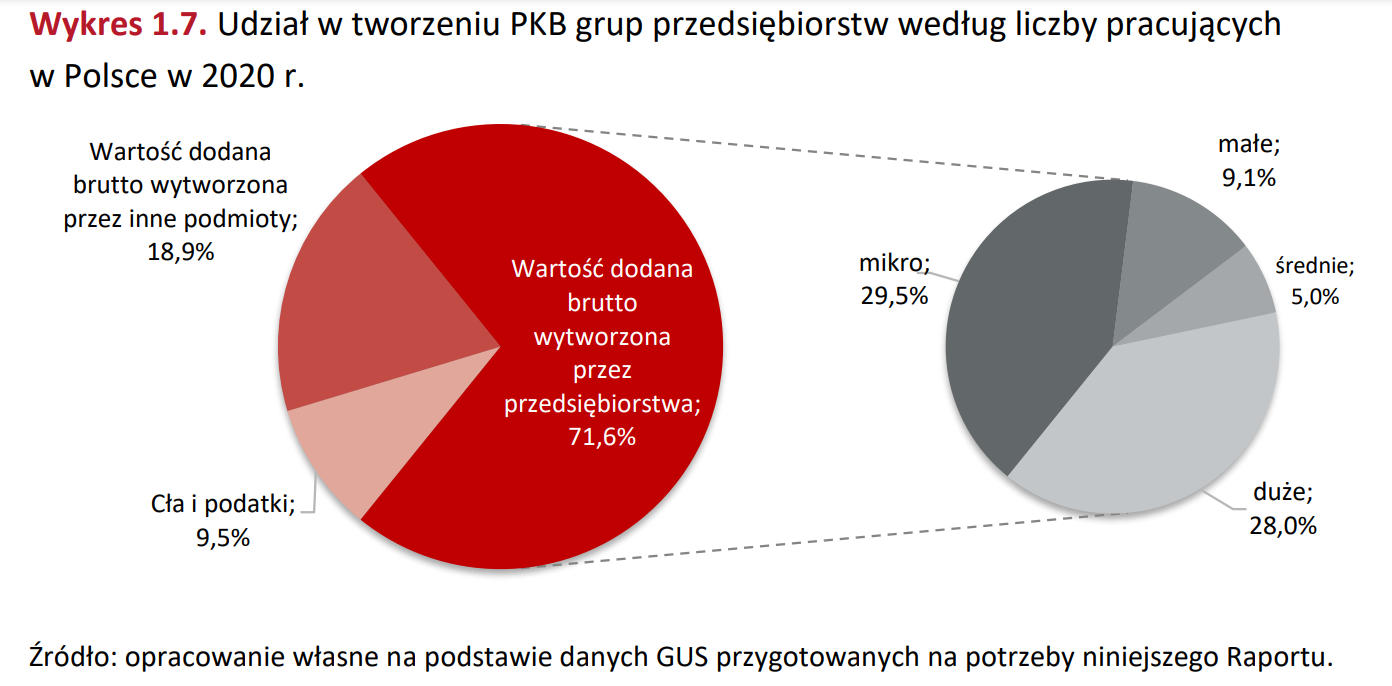
\includegraphics[scale=0.6]{img/udzialMSP.png}
\end{center}

Drugi w kolejności był Handel (23,5\% - MSP; 17,8\% - duże
firmy). Z kolei w dużych przedsiębiorstwach widocznie większy wkład w tworzenie PKB
w porównaniu z sektorem MSP m Przemysł (48,0\% - duże firmy; 17,8\% - MSP),
najmniejszy zaś Budownictwo (3,9\% - duże firmy; 11,8\% - MSP) \cite{RaportPARPoMSP}.

\section*{Sposoby wspierania MŚP w Polsce}

\subsection*{Kredyty preferencyjne}

Jednym ze sposobów wspierania MŚP w Polsce są udzielane przez państwo kredyty preferencyjne.
Według Głównego Urzędu Statystycznego jest to udzielanie kredytów na określone rodzaje działalności,
korzystniejszych wobec określonej grupy kredytobiorców pod względem ogólnych warunków umowy, oprocentowania,
harmonogramu spłat lub innych warunków kredytowania (np. możliwość zastosowania karencji w spłacie kapitału,
stosowania prolongaty w spłacie części albo całości zadłużenia kapitału lub odsetek) \cite{DefKredytPref}.

\medskip

W ostatnich latach kredyty preferencyjne były udzielane przez Bank Gospodarstwa Krajowego (dalej nazywany jako BGK).
Jednym z przykładów programów udzielania kredytów przez BGK jest program pożyczek płynnościowych z
Programu Operacyjnego Inteligentny Rozwój dla mikro, małych i średnich firm.
Ilość pieniędzy przeznaczonych na ten projekt wynosi ponad 4 mld zł. Celem projektu jest wsparcie dla przedsiębiorców z sektora MŚP,
którzy z powodu pandemii COVID-19 znaleźli się w trudnej sytuacji finansowej oraz także dla firm, które mają problemy przez skutki
rosyjskiej agresji wobec Ukrainy \cite{BgkProgramPlynnosci}.

Innym programem BGK jest Kredyt Technologiczny FENG 2021-2027. Jest to dotacja dla mikro-, małych i średnich przedsiębiorstw,
które wdrażają innowacyjną technologię i na jej podstawie rozpoczynają produkcję towarów / świadczenie usług, które są nowe lub znacząco ulepszone.
Planowana kwota dofinansowania wynosi ponad 750 mln złotych \cite{KredytTechnologicznyFENG}.

Warto również tutaj nadmienić, że projekt ten jest finansowany z Programu Fundusze Europejskie dla Nowoczesnej Gospodarki.
Wiele projektów wspierających MŚP jest finansowanych z Funduszy Europejskich dzięki członkostwu Polski w Unii Europejskiej.

\subsection*{Rządowy Program Pierwszy biznes - Wsparcie w starcie}

BGK w swojej działalności wspiera również zakładanie nowych firm. Jednym z programów BGK jest ``Rządowy Program Pierwszy biznes - Wsparcie w starcie''.
Jest to program skierowany m.in. do absolwentów szkół i uczelni wyższych i osób bezrobotnych polegający na użyczeniu przez Bank nisko oprocentowanej
pożyczki na założenie działalności gospodarczej. Pożyczka wynosi około 140 tys. zł (20-krotność przeciętnego wynagrodzenia). Pożyczka jest udzielana na okres do 7 lat,
w tym 12 miesięcy karencji w spłacie kapitału. W ramach tego samego programu zawarta jest również pożyczka na utworzenie miejsca pracy, która wynosi około 42 tys. zł.
(6-krotność przeciętnego wynagrodzenia) \cite{BgkProgramStart}.

Ponadto BGK również wspiera transformację ekologiczną przedsiębiorstw mająch na celu zmniejszenie zużycia energii i instalacji odnawialnych źródeł energii.
Przykładami takich projektów są ``Kredyt ekologiczny'', ``Grant OZE'' czy ``Premia termomodernizacyjna z opcją grantu termomodernizacyjnego'' \cite{BgkProgramEkologia}.

\subsection*{Tarcza antykryzysowa}

W związku z ciężką sytuacją gospodarczą w Polsce spowodowaną pandemią COVID-19, rząd wprowadził tarczę antykryzysową \cite{TarczaAntykryzysowa}.
Celem tarczy antykryzysowej było zapewnienie wsparcia dla przedsiębiorstw, które znalazły się w trudnej sytuacji finansowej.
Wsparcie zostało skierowane m.in. do sektora MŚP, który był najbardziej narażony na skutki wprowadzonych obostrzeń i ograniczeń w gospodarce.
Na pomoc dla przedsiębiorstw przeznaczono ponad 312 mld złotych (w tym 74 mld zł na finansowanie przedsiębiorstw), co stanowiło około 15\% PKB Polski.

Pomoc polegała na wprowadzeniu zwolnień podatkowych, ułatwień w dostępie do kredytów, a także różnych form dotacji czy pożyczek preferencyjnych.
Część tarczy antykryzysowej obejmowała ułatwienia dla przedsiębiorstw w zakresie zatrudniania pracowników,
w tym różnego rodzaju odroczenia składek na ubezpieczenia społeczne czy inne ulgi dla pracodawców.
Tarcza antykryzysowa zawierała także środki pomocowe skierowane do konkretnych sektorów gospodarki, takich jak branża turystyczna czy kultura,
które szczególnie ucierpiały w wyniku ograniczeń związanych z pandemią.
Rząd wprowadził środki wspierające osoby prowadzące działalność gospodarczą na własny rachunek,
zapewniając im wsparcie finansowe w okresie, gdy ich dochody były szczególnie narażone na spadek.
W ramach tarczy antykryzysowej wprowadzono tymczasowe obniżenie stawki VAT dla niektórych branż,
co miało na celu zachęcenie konsumentów do zakupów i wspieranie sektora usługowego.

\subsection*{Wsparcie dla MŚP z Funduszy Europejskich w Polsce}

Polska, będąc aktywnym członkiem Unii Europejskiej, korzysta z różnych instrumentów finansowych dostępnych w ramach Funduszy Europejskich,
aby wspierać rozwój sektora małych i średnich przedsiębiorstw.
Poniżej przedstawione zostały kilka kluczowe aspekty, jakie oferuje to wsparcie \cite{FunduszeEuropejskieMŚP}.

\begin{itemize}
  \item \subsubsection*{Dostęp do Finansowania}
        Fundusze Europejskie umożliwiają MŚP dostęp do różnych źródeł finansowania, takich jak dotacje, pożyczki i inne instrumenty finansowe.
        To otwiera nowe możliwości inwestycyjne i pomaga w finansowaniu projektów rozwojowych.
  \item \subsubsection*{Programy Rozwoju}
        Dzięki wsparciu Funduszy Europejskich, Polska implementuje różnorodne programy rozwoju, które wspierają MŚP w obszarach takich jak innowacje,
        badania i rozwój, czy internacjonalizacja. To sprzyja zwiększaniu konkurencyjności polskich firm na rynku międzynarodowym.
  \item \subsubsection*{Szkolenia i Rozwój Kompetencji}
        Fundusze Europejskie wspierają programy szkoleniowe i rozwój kompetencji pracowników MŚP. Dzięki temu poprawiają się umiejętności zawodowe,
        co wpływa na efektywność i innowacyjność przedsiębiorstw.
  \item \subsubsection*{Integracja z Rynkiem Wspólnotowym}
        Polska, jako członek UE, korzysta z możliwości integracji z rynkiem wspólnotowym. To ułatwia ekspansję MŚP na rynki europejskie,
        tworząc nowe perspektywy handlowe i partnerskie.
\end{itemize}

Listę programów wspierających MŚP tworzonych przez Fundusze Europejskie można znaleźć na stronie
\href{https://www.funduszeeuropejskie.gov.pl/wyszukiwarka/mikro-male-i-srednie-przedsiebiorstwa/}{Programy wsparcia MŚP z Funduszy Europejskich}.

\section*{Rozwiązania podatkowe dla MŚP}

\subsection*{Ulga na start - 6 miesięcy bez składek na ubezpieczenie społeczne}

Jedynm z rozwiązań podatkowych oferowanych przez rząd pozwalających na wspieranie początkowych etapów działalności MŚP jest ulga na start.
Cytat z Ustawy ``Prawo przedsiębiorców'' \cite{PrawoPrzedsiębiorców}:

\begin{itquote}
  ``\textbf{Art. 18. 1.} Przedsiębiorca będący osobą fizyczną, który podejmuje działalność
  gospodarczą po raz pierwszy albo podejmuje ją ponownie po upływie co najmniej
  60 miesięcy od dnia jej ostatniego zawieszenia lub zakończenia i nie wykonuje jej na
  rzecz byłego pracodawcy, na rzecz którego przed dniem rozpoczęcia działalności
  gospodarczej w bieżącym lub w poprzednim roku kalendarzowym wykonywał
  w ramach stosunku pracy lub spółdzielczego stosunku pracy czynności wchodzące
  w zakres wykonywanej działalności gospodarczej, nie podlega obowiązkowym
  ubezpieczeniom społecznym przez okres 6 miesięcy od dnia podjęcia działalności
  gospodarczej.''
\end{itquote}

Dzięki tej uldze, wedle brzmienia artykułu przedsiębiorca może nie płacić składek na ubezpieczenia społeczne
przez 6 miesięcy. Pieniądze, które w ten sposób odłoży może przeznaczyć na początkową działalność przedsiębiorstwa co
wskazuje na proinwestycyjny charakter tego rozwiązania.

\subsubsection*{Ulgi inwestycyjne}

Kolejnym rozwiązaniem podatkowym oferowanym przez rząd są ulgi inwestycyjne.
W 10 maja 2018 roku przez Sejm RP została uchwalona Ustawa o wspieraniu nowych inwestycji \cite{UstawaOInwestycjach}.
Na jej podstawie utworzona została Polska Strefa Inwestycji, która zajmuje się udzielaniem ulg podatkowych przedsiębiorstwom,
które dokonują nowych inwestycji \cite{PolskaStrefaInwestycji}. Według ustawy jest to:
\begin{itemize}
  \item Utworzenie nowego zakładu
  \item Zwiększenie zdolności produkcyjnej
  \item Wprowadzenie produktów dotąd niewytwarzanych
  \item Zasadnicza zmiana dotycząca procesu produkcyjnego
\end{itemize}

Pomoc publiczna oferowania jest przez PSI w sektorach
\begin{itemize}
  \item tradycyjnego przemysłu z wyjątkiem przedsiębiorstw produkujących m.in.: alkohol,
        wyroby tytoniowe, materiały wybuchowe, stal, energię elektryczną i gaz
  \item nowoczesnych usług
\end{itemize}

Na podstawie ustawy o wspieraniu nowych inwestycji przedsiębiorstwa produkcyjne oraz usługowe mogą wnioskować
o zwolnienie od podatku dochodowego CIT lub PIT od realizacji nowej inwestycji.
Wolne od podatku będą dochody uzyskane z działalności gospodarczej określonej w decyzji o wsparciu.
Zwolnienie podatkowe jest przyznawane w formie regionalnej pomocy inwestycyjnej, a jego maksymalne wysokości
wynikają z maksymalnych intensywności pomocy regionalnej wskazanych dla poszczególnych jednostek województw i regionów Polski.
Wysokości maksymalnych intensywności pomocy regionalnej wahają się od 10\% do 50\% w zależności od województwa i regionu Polski.
W przypadku średnich firm maksymalna intensywność pomocy wynosi dodatkowo +10\%, a w przypadku mikro i małych firm +20\%.

Więcej informacji o działalności i oferowanych ulgach przez Polską Strefę Inwestycji można
znaleźć na oficjalnej stronie rządowej pod linkiem: \url{https://www.biznes.gov.pl/pl/polska-strefa-inwestycji}.

\section*{Podsumowanie}

Polska w dzisiejszych czasach oferuje szeroki wachlarz rozwiązań wspierających przedsiębiorczość i rozwój MŚP.
Świadczą o tym rozmaite programy rządowe, które oferują wsparcie finansowe, podatkowe oraz szkolenia i rozwój kompetencji.
Wiele z tych programów jest finansowanych z Funduszy Europejskich, co jest jednym z wielu korzyści płynących z członkostwa Polski w Unii Europejskiej. 
Warto również wspomnieć, że Polska jest jednym z najszybciej rozwijających się krajów w Unii Europejskiej, co jest zasługą m.in.
wspierania przedsiębiorczości i rozwoju MŚP.
Interesem państwa jest wspieranie przedsiębiorczości i rozwoju MŚP, ponieważ jest to jeden z głównych czynników rozwoju gospodarczego kraju.
Z pewnością można stwierdzić, że Polska w dzisiejszych czasach zdecydowanie wspiera przedsiębiorczość i rozwój MŚP.

\pagebreak

\bibliography{bibliography}{}
\bibliographystyle{unsrt}

\end{document}